\section{近似算法}
\subsection{近似算法}
算法$A$是一近似算法 (approximation),$A(I)$是算法$A$在例子$I$的目标函数值,$OPT(I)$是最优解的目标函数值。 \\
算法$A$的近似比$\rho_A = \sup_{I}\{\frac{OPT(I)}{A(I)}, \frac{A(I)}{OPT(I)}\}$。
称算法$A$为$r$近似,在极大化问题中,$\forall I, OPT(I) \le r \times A(I)$;或在极小化问题中,$\forall I, A(I) \le r \times OPT(I)$。

\subsection{背包问题}
假设$s_i$表示物品$i$的所占空间,$v_i$表示物品$i$的价值,$C$表示总共空间,$F_j(i)$表示前$j$个物品中价值和为$i$的物品所需最小空间,有
$$
OPT: argmax \{i | F_j(i) \le c\},F_j(i) = min\{F_{j - 1}(i), F_{j - 1}(i - v_i) + s_i\}
$$
时间复杂度为$O(n^2v_{max})$属于伪多项式时间算法。 \\
若将各个物品的价值缩小$K$倍,$v_i' =  \left\lfloor\frac{v_i}{K}\right\rfloor $,此时时间复杂度变为$O(\frac{n^2v_{max}}{K})$。 \\
令动态规划的解为$S'$,原问题最优解为$S^*$,有
\begin{align}
    \sum_{j \in S'}v_j & \ge \sum_{j \in S'}\left\lfloor\frac{v_j}{K}\right\rfloor \times K \nonumber \\
    & = K \times \sum_{j \in S'}v_j' \nonumber \\
    & \ge K \times \sum_{j \in S^*}v_j'\nonumber \\
    & \ge \sum_{j \in S^*}(\frac{v_j}{K} - 1) \times K \nonumber \\
    & = \sum_{j \in S^*}v_j - K|S^*| \nonumber \\
    & \ge OPT - n \times K \nonumber
\end{align}
希望
\begin{align}
    n \times K &\le \epsilon \times OPT \nonumber \\ 
    & \Rightarrow K \le \frac{\epsilon}{n} \times v_{max} \ \mbox{(因为}OPT \ge v_{max}\mbox{)} \nonumber \\
    & \mbox{(令} K = \frac{\epsilon}{n} \times v_{max} \mbox{)} \nonumber \\
    & \Rightarrow OPT - n \times K = (1 - \epsilon) \times K \nonumber
\end{align}
% 令$K = \frac{\epsilon}{n} \times v_{max}$,$OPT - n \times K = (1 - \epsilon) \times K$,
此时时间复杂度变为$O(\frac{n^2v_{max}}{K}) = O(\frac{n^3}{\epsilon})$。

\subsection{顶点覆盖}
\subsubsection{近似算法$1$}
假设共有 $n$ 个点,$x_i$ 表示第 $i$ 个点是否在答案集合中,$w_i$ 表示第 $i$ 个点的权重,$E$ 表示边集,$(u, v)$ 表示连接点 $u$ 与点 $v$ 的一条边。构造出顶点覆盖 (vertex cover) 模型:
$$
\min \quad \sum_{i = 1}^n w_ix_i
$$
$$
\text{s.t.} 
\begin{cases}
    x_i + x_j \ge 1, \ \forall (i, j) \in E \\
    x \in \{0, 1\}
\end{cases}
$$
这是一个整数规划问题,假设该问题的最优目标函数值为 $\text{OPT}$。 \\
对该问题进行松弛,将 $x \in \{0, 1\}$ 改为 $x \ge 0$。设松弛后的线性规划问题最优解为 $x^*$,最优目标函数值为 $\text{OPT}_{LP}$,有 $\text{OPT}_{LP} \le \text{OPT}$。
构造出原问题的可行解 $x$ 如下:
$$
x_i = \begin{cases} 1 & x^*_i \ge 0.5 \\ 0 & x^*_i < 0.5 \end{cases}
$$ 
由于对于每条边 $(i, j)$ 存在 $x^*_i + x^*_j \ge 1$ 的限制,则 $\max(x^*_i, x^*_j) \ge 0.5$,$x_i + x_j \ge 1$ 仍然成立,此解可行。 \\
有 $x_i \le 2x^*_i$。将构造的可行解代入目标函数,有
$$
\sum_{i=1}^n w_ix_i \le 2\sum_{i=1}^n w_ix^*_i \le 2\text{OPT}_{LP} \le 2\text{OPT}
$$
证明了算法的近似比为 $2$。

\subsubsection{近似算法$2$:原始对偶算法}
有对偶问题:
$$
\max \quad \sum_{e \in E} y_e
$$
$$
\text{s.t.} 
\begin{cases}
    \sum_{i \in e} y_e \le w_i, \ \forall i \in V \\
    y_e \ge 0
\end{cases}
$$
互补松弛条件:
\begin{itemize}
    \item PCS(原始问题的互补松弛条件):$x_i \times (w_i - \sum_{i \in e}y_e) = 0$。
    \item DCS(对偶问题的互补松弛条件):$y_e \times (x_i + x_j - 1) = 0$。
\end{itemize}
若PCS成立,有
$$
\begin{cases}
x_i \ne 0 \Rightarrow w_i = \sum_{i \in e}y_e \\
y_e \ne 0 \Rightarrow 1 \le x_i + x_j \le 2
\end{cases}
$$
则
\begin{align}
    \sum_{i = 1}^nw_ix_i & = \sum_{i = 1}^n (\sum_{i \in e}y_e)x_i \nonumber \\ 
    & \le 2 \times \sum_{e \in E}y_e \nonumber \\
    & \le 2 \times \sum_{i = 1}^n w_ix_i^* \nonumber \\ 
    & \le 2 \times C_{IP}^* \nonumber
\end{align}
算法步骤:
\begin{enumerate}
    \item $x = 0, y = 0$,所有边未标记。
    \item 任选一条未标记的边,提升$y_e$到其某一端点约束变紧。
    \item $x_i = 1$,与$v_i$关联的边全部标记。
    \item 重复上述第二、第三步骤,直到所有边被标记。
\end{enumerate}
假设有以下问题:
\begin{figure}[H]
    \begin{center}
        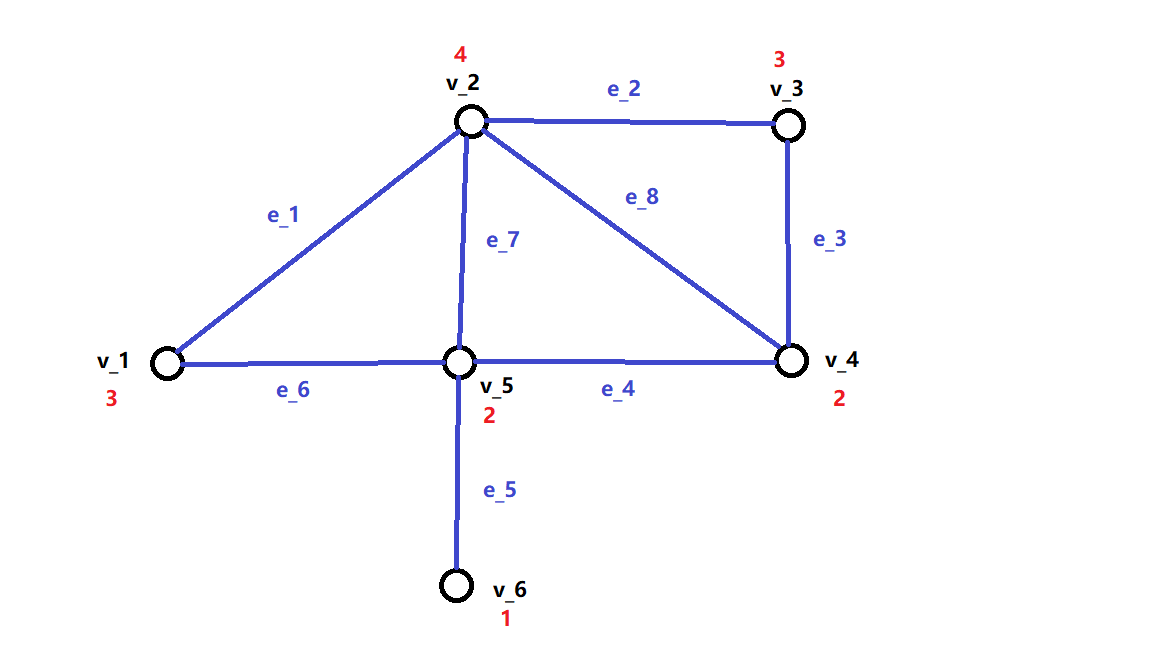
\includegraphics[scale=0.4]{img/vertex_cover.png}
        \caption{顶底覆盖例子。}
    \end{center}
\end{figure}
\begin{enumerate}
    \item 先选$v_1$,提升$e_1 = 3$,$v_1$覆盖,因为$e_6$连接$v_5$,提升$e_6 = 3 - 3 = 0$。
    \item 选择$v_2$,提升$e_2 = 4 - 3 = 1$,$v_2$覆盖,因为$e_7$连接$v_5$,提升$e_7 = 4 - 3 - 1 = 0$;$e_8$连接$v_4$,提升$e_8 =  4 - 3 - 1 - 0 = 0$。
    \item 选择$v_3$,提升$e_3 = 3 - 1 = 2$,$v_3$覆盖。
    \item 选择$v_4$,提升$e_4 = 2 - 0 - 2 = 0$,$v_4$覆盖。
    \item 选择$v_6$,提升$e_5 = 1$,$v_6$覆盖。
\end{enumerate}
得到原问题权重:$13$(点);对偶问题权重:$7$(边)。
\begin{figure}[H]
    \begin{center}
        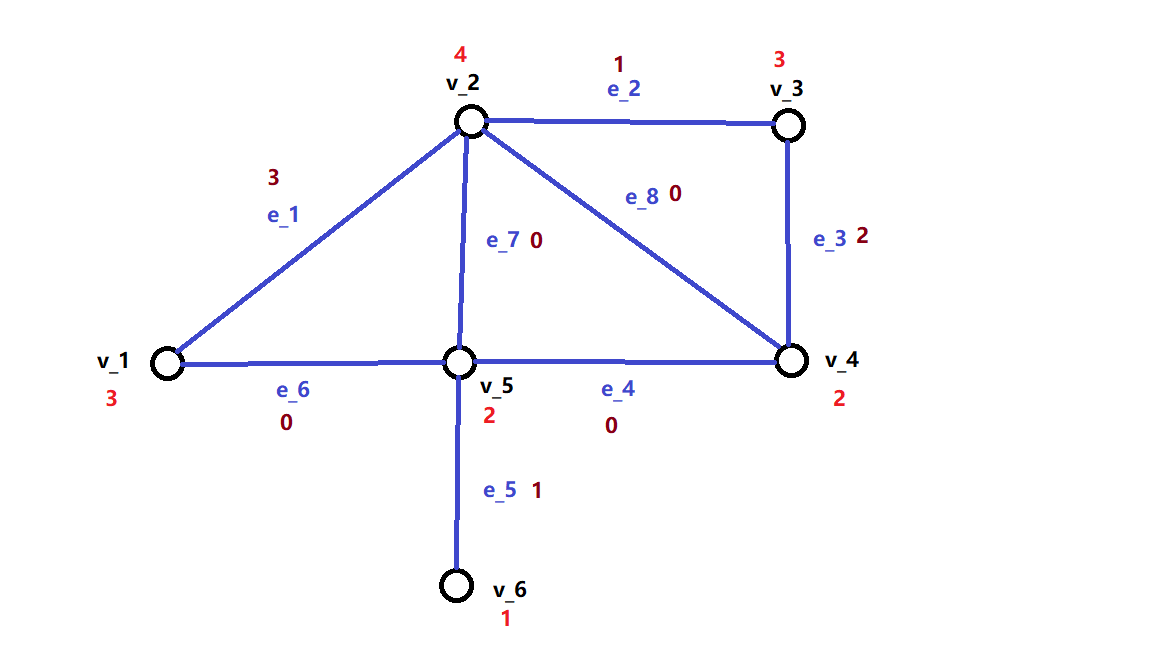
\includegraphics[scale=0.5]{img/vertex_cover_result.png}
        \caption{顶底覆盖例子结果。}
    \end{center}
\end{figure}

\subsection{非等同并行机调度}
有 $m$ 台机器和 $n$ 件物品,每件物品都要在一台机器上加工,$a_{i, j}$表示第 $i$ 台机器加工第 $j$ 件物品的时间。求一种把物品分配给机器的方案,使得加工总时长最长的机器,加工总时长最短,即为非等同并行机调度 (Unrelated Parallel Machine Scheduling, UPMS)。
构造出模型:
$$
\min \quad T
$$
$$
\text{s.t.} 
\begin{cases}
    \sum_{i = 1}^m x_{i, j} = 1, \ \forall j \in \{1, 2, \ \cdots, n\} \\
    \sum_{j = 1}^n a_{i, j}x_{i, j} \le T, \ \forall i \in \{1, 2, \ \cdots, m\} \\
    x_{i, j} \in \{0, 1\}
\end{cases}
$$
此模型不适合进行松弛。假设只有一件物品需要加工,且该物品在所有机器上的加工时间都为 $1$,则原问题的最优目标函数值为 $1$,然而松弛求出的最优解为 $x_{i, 1} = 1/m$,下界不够紧,难以进行近似比分析。 \\~\\
先二分 $T$ 。若 $a_{i, j} > T$,加上 $x_{i, j} = 0$ 的限制,让改动后的问题存在可行解的最小的 $T$,就是原问题最优目标函数值的下界(可利用两阶段法的第一阶段判断是否存在可行解)。 \\
假设改动后的问题最优解为 $x^*$,对于第 $j$ 件物品,若 $\exists i, x^*_{i, j} = 1$ ,则称该物品为“整数物品”,否则称该物品为“分数物品”,假设共有 $n_1$ 个“整数物品”, $n_2$ 个“分数物品”。有 $n_1 + n_2 = n$, 若第 $j$ 件物品为“分数物品”, $x_{i, j}$ 中至少有两个非零值。
由于原问题有 $n + m$ 条限制,根据单纯形法,非零的变量至多有 $n + m$ 个,有 $n_1 + 2n_2 \le n + m$,得到 $n_2 \le m$。 \\~\\
通过使得每台机器的加工总时长都不超过 $2T$,设计一个近似比为 $2$ 的算法。 \\
定义:若连通图中边数小等于点数,称该连通图为伪树;若一张图的所有连通块都是伪树,称该图为伪森林。 \\
构造一张二分图:左边有 $m$ 个点,每个点表示一台机器;右边有 $n$ 个点,每个点表示一件物品。若 $x_{i, j} > 0$ 则连接第 $i$ 台机器和第 $j$ 件物品。如果这个二分图不连通,那么对每个连通块分别求解,最后将解合并即为答案,因此可以假设该二分图连通。由于非零变量至多有 $n+m$ 个,所以该连通图的边数不超过点数,是一个伪树。 
首先考虑“整数物品”。每个“整数物品” $j$ 都只和一台机器 $i$ 有连边 $(i, j)$,将“整数物品” $j$ 放在机器 $i$ 中加工,并去掉物品 $j$ 和边 $(i, j)$。由于每次恰好去除一个点和一条边,这张图仍然是伪树。此时每台机器的加工总时长至多为 $T$,否则问题的最优目标函数值就会超过 $T$ 。 \\
此时,仅剩机器和“分数物品”了。考虑所有度数为 $1$ 的机器 $i$。假设唯一连接机器 $i$ 的边是 $(i, j)$,将“分数物品” $j$ 放在机器 $i$ 中加工,并去掉机器 $i$、物品 $j$ 和物品 $j$ 的所有连边。由于每件“分数物品”都有至少两条连边,所以我们每次都会去掉两个点以及至少两条边,可知剩下的图是伪森林。
反复删除度数为 $1$ 的机器,直到最后不存在度数为 $1$ 的机器为止。 \\
由于剩下的图是伪森林也是二分图,则剩下的图中只能包含若干偶环,在偶环上任意给每台机器分配一件物品即可。 \\
因此,每台机器至多分配到一个“分数物品”,再加上原来分配给它的“整数物品”,每台机器的总加工时长至多为 $2T$,得到一个近似比为 $2$ 的算法。

\subsection{装箱问题}
\subsubsection{均摊体积}
假设第 $i$ 件物品体积为 $a_i$,定义权重 $w(a_i)$ :
$$
w(a_i) = \frac{6}{5}a_i + v(a_i)
$$
称 $v$ 为 bonus,定义为:
$$
v(a_i) = \begin{cases} 0 & a_i \le \frac{1}{6} \\ \frac{3}{5}(a_i - \frac{1}{6}) & \frac{1}{6} < a_i \le \frac{1}{3} \\ \frac{1}{10} & \frac{1}{3} < a_i \le \frac{1}{2} \\ \frac{2}{5} & a_i > \frac{1}{2} \end{cases}
$$
记 $w(I)$ 为装箱问题 (bin packing)的一个实例 $I$ 的权重总和,$\text{FF}(I)$ 表示对实例 $I$ 运用 First fit 算法得到的目标函数值,$\text{OPT}(I)$ 表示实例 $I$ 的最优目标函数值。
再记 $B$ 为 first fit 算法得到的方案,$B^*$ 为最优方案,$c(B_j)$ 表示第 $j$ 个 bin 中物品的体积总和,$w(B_j)$ 表示第 $j$ 个 bin 中物品的权重总和,有
$$
w(I) = \sum\limits_{i=1}^n w(a_i) = \sum\limits_{j=1}^{\text{FF}(I)}w(B_j) = \sum\limits_{j=1}^{\text{OPT}(I)}w(B^*_j)
$$
先是证明均摊体积不超过$1.7$。 \\
对于一个箱子,可分以下情况讨论:
\begin{enumerate}
    \item 所有物品体积 $c$ 均有 $c \le \frac{1}{6}$。箱子的权重就是箱中物品体积总和的 $1.2$ 倍,不会超过 $1.7$。
    \item 存在物品体积 $c$ 有 $\frac{1}{6} < c \le \frac{1}{2}$。这种物品在一个箱中至多有 $5$ 个,bonus 不会超过 $\frac{1}{10} \times 5 = \frac{1}{2}$,权重也不会超过 $1.7$。
    \item 存在两个物品体积 $c_1$ 和 $c_2$ 有 $c_1 > \frac{1}{2}$ 且 $\frac{1}{3} < c_2 \le \frac{1}{2}$。其它物品的体积都不会超过 $\frac{1}{6}$,没有 bonus;$c_1$ 和 $c_2$ 带来的 bonus 恰为 $0.5$,权重不会超过 $1.7$。
    \item 存在三个物品体积 $c_1$,$c_2$ 和 $c_3$ 有 $c_1 > \frac{1}{2}$,$\frac{1}{6} < c_2, c_3 \le \frac{1}{3}$ 且 $c_2 + c_3 < \frac{1}{2}$。其它物品的体积都不会超过 $\frac{1}{6}$,没有 bonus;$c_2$ 和 $c_3$ 带来的 bonus 为 $\frac{3}{5}(c_2 - \frac{1}{6}) + \frac{3}{5}(c_3 - \frac{1}{6}) < 0.1$,再加上 $c_1$ 带来的 bonus $0.4$,权重不会超过 $1.7$。
\end{enumerate}
证明了均摊体积不超过$1.7$。 \\~\\
接着证明除两个箱子外,其它箱子的权值均值至少为$1$。
首先去掉权值至少为 $1$ 的箱子,考虑权值不足 $1$ 的箱子。可知权值不足 $1$ 的箱子有以下性质:
\begin{enumerate}
    \item 不含体积至少为 $0.5$ 的物品,因为若含体积大于$0.5$的物品,该物品的权重就会超过$1$。
    \item 一个箱中不会包含两个体积至少为 $\frac{1}{3}$ 的物品,因为若含两个体积大于$\frac{1}{3}$的物品,该两个物品的权重就会超过$1$。
    \item 箱子的体积之和小于 $\frac{5}{6}$,因为若箱子的体积之和大于$\frac{5}{6}$,不算bonus就足以使权重超过$1$。
\end{enumerate}
可得
\begin{enumerate}
    \item 除了最后一个箱子,其它箱子中至少有两个物品。
    \item 除了最后两个箱子,其它箱子的体积之和都大于 $\frac{2}{3}$(如果有一个 bin 的体积之和不超过 $\frac{2}{3}$,由于是 First fit 算法,后面的箱子里的物品体积至少为 $\frac{1}{3}$ 但少于 $\frac{1}{2}$;而后面至少还有两个箱子,违反了“一个箱子内不会包含两个体积至少为 $\frac{1}{3}$ 的物品”的性质)。
\end{enumerate}
再来证明一个引理:如果两个箱子 $B_1$ 和 $B_2$ 满足 $B_1$ 在 $B_2$ 前面、$w(B_1), w(B_2) < 1$、$c(B_1) \ge \frac{2}{3}$ 以及 $B_2$ 有至少两个物品,则 $\frac{6}{5}c(B_1) + v(B_2) \ge 1$。 \\
有以下性质:
\begin{enumerate}
    \item $c' \ge \frac{1}{6}$,否则 $B_1$ 将会与“箱子的体积之和小于 $\frac{5}{6}$”的性质矛盾。
    \item $ c' < \frac{1}{3}$,否则 $B_2$ 将会与“一个箱子中不会包含两个体积至少为 $\frac{1}{3}$ 的物品”的性质矛盾。
    \item $c' > 1 - c(B_1)$,否则 $c'$ 就会放进 $B_1$ 。
\end{enumerate}
得到 $\frac{1}{6} \le c' < \frac{1}{3}$,则
\begin{align}
    \frac{6}{5}c(B_1) + v(B_2) & \ge \frac{6}{5}c(B_1) + 2 \times v(c') \nonumber \\ 
    & > \frac{6}{5}c(B_1) + \frac{6}{5}(1 - c(B_1) - \frac{1}{6}) \nonumber \\ 
    & = 1 \nonumber
\end{align}
假设 First fit 算法得到的方案中,权重之和小于 $1$ 的箱子按先后顺序为 $B_1, B_2, \dots, B_k$,则
\begin{equation}
\begin{split}
    & w(B_1) + w(B_2) + \dots + w(B_{k-2}) + w(B_{k-1}) + w(B_k) \nonumber \\ 
    = & \ v(B_1) + (\frac{6}{5}c(B_1) + v(B_2)) + \dots + (\frac{6}{5}c(B_{k-2}) + v(B_{k-1})) \nonumber \\
    + & \ (\frac{6}{5}c(B_{k-1}) + \frac{6}{5}c(B_k)) + v(B_k) \nonumber \\ 
    \ge & \ (k-2) + \frac{6}{5} \nonumber
\end{split}
\end{equation}
即除了最后两个箱子,其它的箱子权值均值都至少为$1$,再加上$0.8$以及权值至少为 $1$ 的箱子,则所有的箱子的权值均值就都至少为 $1$。证明First fit算法有 $1.7$ 的近似比。

\subsection{旅行商问题}
在满足三角不等式的完全图上,旅行商问题 (Travelling Salesman Problem, TSP),可通过搜索最小生成树 (Minimum Spanning Tree, MST),将树上每条边重复一次变成欧拉图 (Euler graph),在欧拉图上 short-cutting,得到近似比为 $2$的上界。 \\
下面证明近似比为$1.5$的近似算法: \\
将树上度数为奇数的点进行配对(一张图上度数为奇数的点有偶数个),每一对之间连一条边,则构成的图上的点的度数都是偶数,即为欧拉图。 \\
\begin{figure}[H]
    \begin{center}
        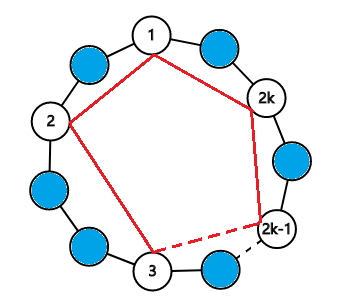
\includegraphics[scale=0.8]{img/tsp.png}
        \caption{度数为奇数的点匹配示意图。}
        \label{img:tsp}
    \end{center}
\end{figure}
在图\ref{img:tsp} 上,白色的点是最小生成树上的度数为奇数的点。将奇点按顺序进行 short-cutting,得到两个不相交匹配($1 - 2, 3 - 4, \cdots, (2k - 1) - 2k$ 以及 $2 - 3, 4 - 5, \cdots, 2k - 1$)。由于满足三角不等式,这两个匹配的权值之和不大于 $\text{OPT}$,则两个匹配中较小的权值不大于 $0.5\text{OPT}$。因为算法中求出的是最小完美匹配,则最小完美匹配的权值也不大于 $0.5\text{OPT}$。
因此,最小生成树和最小权完美匹配证明了 $1.5$ 的近似比。
\begin{figure}[H]
    \begin{center}
        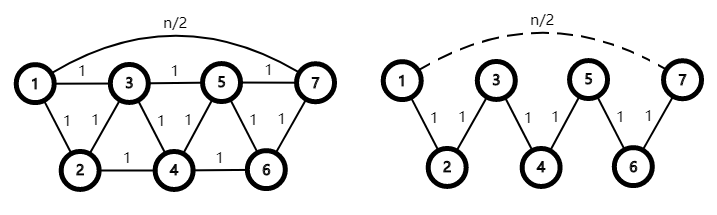
\includegraphics[scale=0.8]{img/tsp_2.png}
        \caption{最小权完美匹配示意图。}
        \label{img:tsp_2}
    \end{center}
\end{figure}
图\ref{img:tsp_2} 可说明近似比$1.5$是紧的。途中没有画出来的边权值都是 $2$,右图实线是算法可能获得的最小生成树,虚线是算法可能算出的最小权完美匹配。可得最优解为 $n$,而算法可能得出的解是 $n + \frac{n}{2}$。 \\
只要“梯形”上面的点足够多,则近似比为 $1.5$。

\subsubsection{满足三角不等式的完全图的最短哈密尔顿路}
在满足三角不等式的完全图中,求最短哈密尔顿路 (shortest Hamiltonian path)。
算法步骤:
\begin{enumerate}
    \item 求个最小生成树 $T$。假设$S$为在最小生成树上度数为奇数的点的集合。
    \item 求 $S$ 的最小权匹配 $M$。假设最优解上有 $2t$ 个度数为奇数的点,则可以拆成两个匹配:$1 - 2, 3 - 4, \cdots, (2t - 3) - (2t - 2)$($(2t - 1)$ 和 $2t$ 没有匹配) 与 $2 - 3, 4 - 5, 6 - 7, \cdots, (2t - 2) - (2t - 1)$($1$ 和 $2t$ 没有匹配,其中$u - v$表示点$u$和点$v$匹配),可以证明 $M$ 的权值之和至多为 $0.5\text{OPT}$。
    \item $T \cup M$ 即为一张有欧拉路 (Euler path)的图,通过 short-cutting 把欧拉路变成哈密尔顿路即可。
\end{enumerate}
此算法的近似比为$1.5$。

\subsubsection{与哈密尔顿圈相关的优化问题}
\begin{itemize}
    \item 最长哈密尔顿路 (Longest Hamiltonian path)。
    \item 最小圈覆盖 (Minimum cycle cover problem, MCCP).
    \item 最小双联通子图 (Minimum biconnected subgraph(边数最少)).
    \item 最小分支双联通子图 (Minimum branch biconnected subgraph).
    \item 最大内部生成树 (Maximum internal spanning tree(叶子节点最少)).
\end{itemize}

\pagebreak
